\documentclass[10pt]{beamer}
\usepackage{mystyle}
\usepackage{pythonhighlight}

\date{September 2021}

\title{CycleGAN}
\AtBeginDocument{\subtitle{ISPR - Midterm 4}}


\NewDocumentCommand{\XX}{}{\mathcal{X}}
\NewDocumentCommand{\YY}{}{\mathcal{Y}}
\NewDocumentCommand{\LL}{}{\mathcal{L}}
\NewDocumentCommand{\EE}{}{\mathbb{E}}

\graphicspath{{pictures/}}

\tikzset{
pics/image/.style n args={3}{code={
	\node[drop shadow={shadow xshift=1pt,shadow yshift=-1pt}] (-image)[inner sep=0pt,#3]{\includegraphics[keepaspectratio,#2]{#1}};
	\draw[black,thin] (-image.north west) rectangle (-image.south east);
}},
myarrow/.style={-{Latex[open,line width=1pt,length=15pt 0]},mythemecolor,line width=5pt,shorten <=3pt,shorten >=3pt,postaction={draw=white,line width=3pt,-,shorten <=4pt,shorten >=15pt}}
}

\begin{document}

\frame{\titlepage}

\begin{frame}[fragile]{Task}{Unsupervised domain translation}
\def\inlineimage#1{\tikz[baseline=-3pt]\pic{image={#1}{height=1em}{}};}
Given samples $\{\inlineimage{conditional-input},\inlineimage{unsupervised-input},\ldots\}\subseteq\XX$ and $\{\inlineimage{unsupervised-output-1},\inlineimage{unsupervised-output-2},\ldots\}\subseteq\YY$ from two different domains, learn a mapping
\[
\map{G}{\XX}{\YY}
\]
such that $\hat{y}\coloneqq G(x)$ is indistinguishable from $y\in \YY$.
\def\imageh{1cm}
\tikzset{node distance=1.5cm}
\begin{itemize}
\item \textbf{Conditional generation:} the output $\hat{y}\in\YY$ should retain some features of the input $x\in\XX$.
\begin{center}
\begin{tikzpicture}[start chain,label distance=.4cm,every label/.style={anchor=base}]
\pic{image={conditional-input}{height=\imageh}{on chain,label={below:$x$}}};
\pic{image={conditional-output}{height=\imageh}{on chain,label={below:$\hat{y}$},join=by myarrow}};
\pic[node distance=.5cm] (a) {image={conditional-output-no}{height=\imageh}{on chain,opacity=.8}};
\begin{scope}[transparency group,opacity=.7]
\draw[red,line width=4pt,preaction={draw=white,line width=6pt,line cap=round}] (a-image.south west) -- (a-image.north east) (a-image.north west) -- (a-image.south east);
\end{scope}
\end{tikzpicture}\vspace{-.2cm}
\end{center}
\item \textbf{Unpaired samples:} the expected output $\hat{y}_i$ for a specific sample $x_i\in\XX$ is unknown even at training time.
\begin{center}
\begin{tikzpicture}[start chain,label distance=.4cm,every label/.style={anchor=base}]
\pic{image={unsupervised-input}{height=\imageh}{on chain,label={below:$x_i$}}};
\node[draw=black,fill=gray!50,on chain,drop shadow={shadow xshift=1pt,shadow yshift=-1pt},join=by myarrow,label={below:$\hat{y}_i$},font=\bfseries\huge,minimum height=\imageh,minimum width={1.33*\imageh}] {?};
\pic[node distance=.5cm] (a) {image={unsupervised-output-1}{height={.4cm}}{on chain}};
\tikzset{node distance=.1cm}
\pic {image={unsupervised-output-2}{height=.4cm}{above=of a-image}};
\pic {image={unsupervised-output-3}{height=.4cm}{below=of a-image}};
\end{tikzpicture}\vspace{-.2cm}
\end{center}
\end{itemize}
\end{frame}

\begin{frame}[fragile]{Loss function}{The innovation of cycle-consistency}
\faLightbulb \textbf{Idea:} train two generators $\map{G}{\XX}{\YY}$ and $\map{F}{\YY}{\XX}$ simultaneously.

\tikzset{
pics/domain/.style 2 args={code={
	\node[minimum width=1.33cm,minimum height=1.33cm,anchor=south west] (-bbox) {};
	\draw[gray!50,decorate,decoration={zigzag,amplitude=.2mm}] (-bbox.north west) rectangle (-bbox.south east);
	\node[anchor=#2,black!70] at (-bbox.#2) {#1};
}},
picture with domains/.style={
x sample/.style={circle,draw=black,fill=blue!70!cyan,inner sep=.3mm},
y sample/.style={x sample,fill=red},
every edge/.style={draw,-{Latex},shorten <=.6mm,shorten >=.6mm},
show distance/.style={draw=violet,|/.tip={Rays[n=2,width=1mm]},>={Classical TikZ Rightarrow[width=1mm]},|<->|,decorate,decoration={simple line,raise=-1.2mm}}
}}
\pgfdeclaredecoration{simple line}{initial}{
  \state{initial}[width=\pgfdecoratedpathlength-1sp]{\pgfmoveto{\pgfpointorigin}}
  \state{final}{\pgflineto{\pgfpointorigin}}
}
\begin{center}
\def\arraystretch{1.5}
\begin{tabularx}{\textwidth}{@{}X!{\color{gray!50}\vrule}X!{\color{gray!50}\vrule}X@{}}
\textcolor{mythemecolor}{GAN architecture}&\textcolor{mythemecolor}{Cycle-consistency}&\textcolor{mythemecolor}{Identity regularization}\\
\makecell[c]{
\begin{tikzpicture}[
node data/.style={draw=orange!30!gray,fill=orange!30,inner xsep=1mm,inner ysep=.5mm,text height={height("l")},text depth={depth("y")}},
node model/.style={draw=cyan!20!gray,fill=cyan!20,rounded corners=1.5,inner sep=1mm,text height={height("l")},text depth={depth("y")}},
every new ->/.style={gray,-{Latex[scale=.6]}}
]
\graph[grow right sep=2mm,math nodes,simple] {
x [node data] -> G [node model] -!- {hy/\hat{y} [node data], y [node data]} -> /D_{\YY} [y=-.5,node model] -> {[nodes={violet,font=\tiny,inner xsep=0mm}] /\text{fake?} [y=-.1],/\text{real?} [y=.1]};
G -> hy;
};
\end{tikzpicture}
}&
\makecell[c]{
\begin{tikzpicture}[picture with domains]
\pic {domain={$\XX$}{north west}};
\node[x sample] (x) at (.6,.8) {};
\node[x sample] (z) at (.8,.4) {};
\begin{scope}[shift={(1.7,0)}]arrows.meta
\pic {domain={$\YY$}{north east}};
\node[y sample] (y) at (.6,.6) {};
\end{scope}
\path (x) edge[bend left] node[above] {$G$} (y) (y) edge[bend left] node[below] {$F$} (z);
\path[show distance] (x.center) -- (z.center);
\end{tikzpicture}
}&
\makecell[c]{
\begin{tikzpicture}[picture with domains]
\pic {domain={$\YY$}{north east}};
\begin{pgfinterruptboundingbox}
\path[every edge] (.4,1.) node[y sample] (y1) {} to[bend right=120,min distance=1.25cm,"$G$"'] (.6,.6) node[y sample] (y2) {};
\end{pgfinterruptboundingbox}
\path[show distance] (y2.center) -- (y1.center);
\end{tikzpicture}
}
\\
\faChartLine{} $G(x)\approx y$&\faChartLine{} $F\circ G=\operatorname{id}_{\XX}$&\faChartLine{} $G(y)=y$
\end{tabularx}
\end{center}
\setlength{\abovedisplayskip}{0pt}
\setlength{\belowdisplayskip}{0pt}
\begin{align*}
\textcolor{violet}{\LL}={}&\tikzmarknode{l1}{\EE_{x\sim p(x)}[\log(1-D_{\YY}(G(x)))]+\EE_{y\sim p(y)}[\log D_{\YY}(y)]}&\quad&\tikzmarknode[violet]{r1}{\LL_{\text{adv}}(G,D_{\YY})}\\
{}+{}&\tikzmarknode{l2}{\EE_{y\sim p(y)}[\log(1-D_{\XX}(F(y)))]+\EE_{x\sim p(x)}[\log D_{\XX}(x)]}&&\tikzmarknode[violet]{r2}{\LL_{\text{adv}}(F,D_{\XX})}\\
{}+{}&\tikzmarknode{l3}{\lambda\cdot\EE_{x\sim p(x)}[\norm{F(G(x))-x}_1]}&&\tikzmarknode[violet]{r3}{\LL_{\text{cyc}}(F\circ G)}\\
{}+{}&\tikzmarknode{l4}{\lambda\cdot\EE_{y\sim p(y)}[\norm{G(F(y))-y}_1]}&&\tikzmarknode[violet]{r4}{\LL_{\text{cyc}}(G\circ F)}\\
{}+{}&\tikzmarknode{l5}{\alpha\cdot\EE_{y\sim p(y)}[\norm{G(y)-y}_1]}&&\tikzmarknode[violet]{r5}{\LL_{\text{id}}(G)}\\
{}+{}&\tikzmarknode{l6}{\alpha\cdot\EE_{x\sim p(x)}[\norm{F(x)-x}_1]}&&\tikzmarknode[violet]{r6}{\LL_{\text{id}}(F)}
\begin{tikzpicture}[overlay,remember picture]
\foreach \i[evaluate=\i as \i using int(\i)] in {1,...,6} {
\draw[shorten <=1mm,shorten >=1mm,violet!40,dashed] (r\i) -- (l\i);
}
\end{tikzpicture}
\end{align*}
\end{frame}

\begin{frame}{Model}{Architectures of the generators and the discriminators}
\begin{tabularx}{\textwidth}{@{}lY@{}}
\makecell[l]{$G,F$}&\makecell[l]{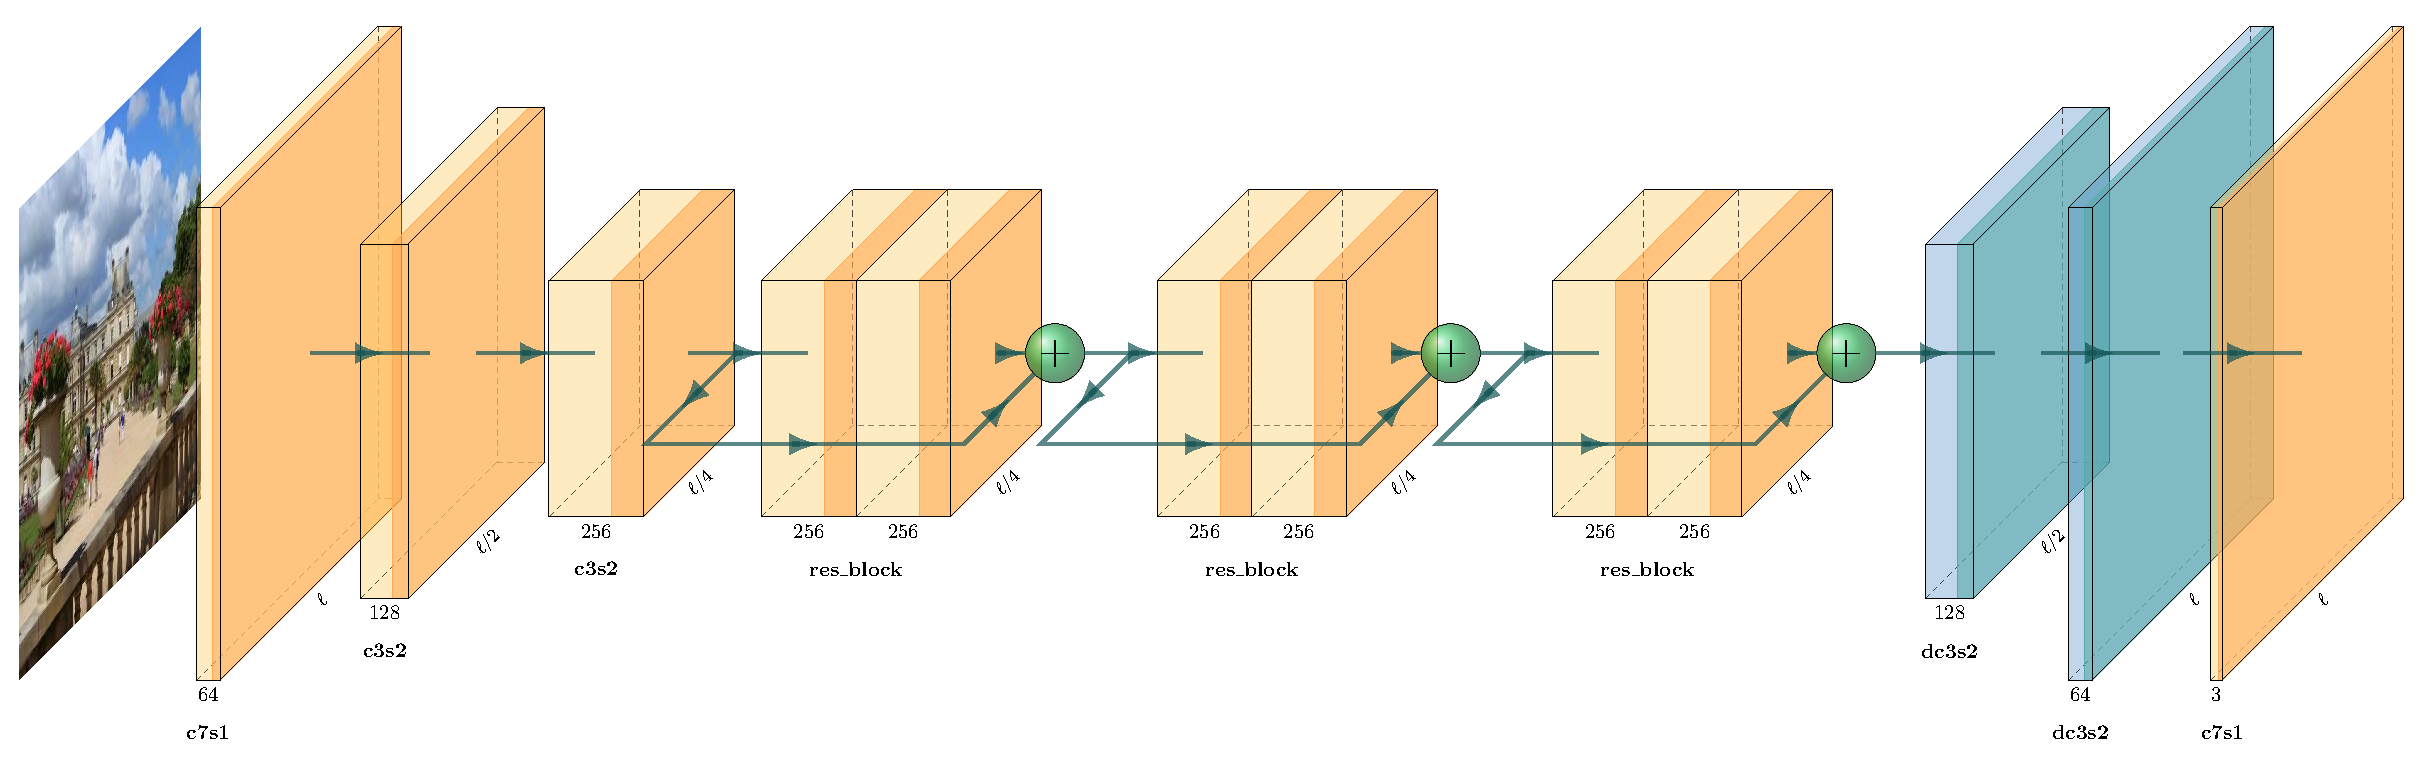
\includegraphics[height=.3\textheight]{generator}}\\
\makecell[l]{$D_{\XX},D_{\YY}$}&\makecell[l]{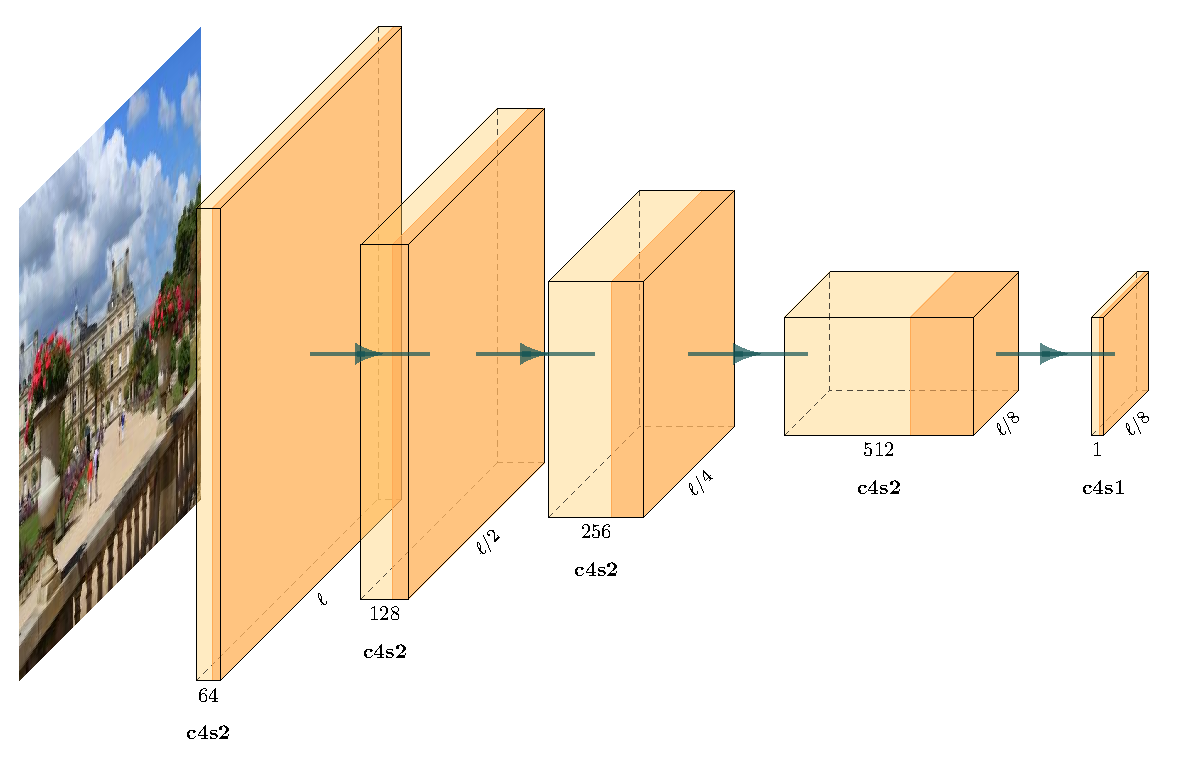
\includegraphics[height=.3\textheight]{discriminator}}
\end{tabularx}
\end{frame}

\begin{frame}[fragile]{Results}
\def\imagew{1.8cm}
\setlength{\tabcolsep}{5pt}
\def\resrow#1{\makecell[c]{\tikz\pic{image={res-#1-1}{width=\imagew}{}};}&\makecell[c]{\tikz\pic{image={res-#1-2}{width=\imagew}{}};}&\makecell[c]{\tikz\pic{image={res-#1-3}{width=\imagew}{}};}}
\begin{tabularx}{\textwidth}{@{}Xccc@{}}
&$x$&$G(x)$&$F(G(x))$\\[1mm]
\makecell[l]{\usebeamertemplate{itemize item} Photo $\to$ Cezanne}&\resrow{1}\\
\makecell[l]{\usebeamertemplate{itemize item} Horse $\to$ Zebra}&\resrow{2}\\
\makecell[l]{\usebeamertemplate{itemize item} Winter $\to$ Summer}&\resrow{3}\\
\makecell[l]{\usebeamertemplate{itemize item} Aerial photo $\to$ Grid view}&\resrow{4}
\end{tabularx}
\end{frame}

\begin{frame}{Conclusion}{Strengths and weaknesses}
\begin{block}{Pros}
\begin{itemize}
\item Multi-purpose image-to-image domain translation.
\item Fully unsupervised model.
\end{itemize}
\end{block}

\begin{block}{Cons}
\def\imageh{1.2cm}
\tikzset{every picture/.style={remember picture}}
\begin{itemize}
\item Failure to adapt to unseen contexts.
\begin{center}
\begin{tabularx}{\linewidth}{@{}YY@{\hspace{1.8cm}}YY@{}}
Zebra&Horse&Apple&Orange\\
\tikz\pic (zebra) {image={fail-unseen-3}{height=\imageh}{}};&\tikz\pic (horse) {image={fail-unseen-4}{height=\imageh}{}};&\tikz\pic (apple) {image={fail-unseen-1}{height=\imageh}{}};&\tikz\pic (orange) {image={fail-unseen-2}{height=\imageh}{}};
\end{tabularx}
\end{center}
\item Only suitable for texture/style changes.
\begin{center}
\begin{tabularx}{\linewidth}{@{}YY@{\hspace{1.8cm}}YY@{}}
Dog&Cat&Cat&Dog\\
\tikz\pic (dog-in) {image={fail-geom-1}{height=\imageh}{}};&\tikz\pic (cat-out) {image={fail-geom-2}{height=\imageh}{}};&\tikz\pic (cat-in) {image={fail-geom-3}{height=\imageh}{}};&\tikz\pic (dog-out) {image={fail-geom-4}{height=\imageh}{}};
\end{tabularx}
\end{center}
\end{itemize}
\end{block}
\tikz[overlay,remember picture]\foreach \from/\to in {zebra/horse,apple/orange,dog-in/cat-out,cat-in/dog-out} \draw[myarrow] (\from-image) to (\to-image);
\end{frame}

\end{document}